\documentclass[12pt]{report}
\usepackage[utf8]{inputenc}
\usepackage[T2A]{fontenc}
\usepackage[russian]{babel}

\usepackage{amsmath,amsfonts,amssymb,amsthm,mathtools}
\DeclarePairedDelimiter\abs{\lvert}{\rvert}

\usepackage{pgfplots}
\usepackage{filecontents}
\usepackage{indentfirst}
\usepackage{eucal}
\usepackage{enumitem}
% Для \abs{}
\usepackage{commath}
\usepackage{float}
\frenchspacing

% Для нормальных переносов
\sloppy

\usetikzlibrary{datavisualization}
\usetikzlibrary{datavisualization.formats.functions}

\usepackage[left=2cm,right=2cm, top=2cm,bottom=2cm,bindingoffset=0cm]{geometry}
% Для измененных титулов глав:
\usepackage{titlesec, blindtext, color} % подключаем нужные пакеты
\definecolor{gray75}{gray}{0.75} % определяем цвет
\newcommand{\hsp}{\hspace{20pt}} % длина линии в 20pt
% titleformat определяет стиль
\titleformat{\chapter}[hang]{\Huge\bfseries}{\thechapter\hsp\textcolor{gray75}{|}\hsp}{0pt}{\Huge\bfseries}

% plot
\usepackage{xcolor}
\usepackage{stmaryrd}
\usepackage{wasysym}
\usetikzlibrary{datavisualization}
\usetikzlibrary{datavisualization.formats.functions}

% листинги
\usepackage{listings}
\usepackage{graphicx}
\usepackage{caption}
\usepackage{textcomp}
\lstset{
    language = C,
    basicstyle=\small\sffamily,
    numbers=left,
    numberstyle=\tiny,
    stepnumber=1,
    numbersep=5pt,
    showspaces=false,
    showstringspaces=false,
    showtabs=false,
    frame=single,
    tabsize=2,
    captionpos=t,
    breaklines=true,
    breakatwhitespace=false,
    escapeinside={\#*}{*)}
}
\captionsetup[lstlisting]{justification=raggedright, singlelinecheck=off}

\begin{document}
%\def\chaptername{} % убирает "Глава"
    % Титульник
\thispagestyle{empty}
\begin{titlepage}
	\noindent \begin{minipage}{0.15\textwidth}
				  
\includegraphics[width=\linewidth]{img/b_logo}
	\end{minipage}
	\noindent\begin{minipage}{0.9\textwidth}
				 \centering
				 \textbf{Министерство науки и высшего образования Российской Федерации}\\
				 \textbf{Федеральное государственное бюджетное образовательное учреждение высшего образования}\\
				 \textbf{~~~«Московский государственный технический университет имени Н.Э.~Баумана}\\
				 \textbf{(национальный исследовательский университет)»}\\
				 \textbf{(МГТУ им. Н.Э.~Баумана)}
	\end{minipage}

	\noindent\rule{18cm}{3pt}
	\newline\newline
	\noindent ФАКУЛЬТЕТ $\underline{\text{«Информатика и системы управления»}}$ \newline\newline
	\noindent КАФЕДРА $\underline{\text{«Программное обеспечение ЭВМ и информационные технологии»}}$\newline\newline\newline\newline\newline


	\begin{center}
		\noindent\begin{minipage}{1.3\textwidth}
					 \centering
					 \Large\textbf{  Отчет по лабораторной работе №4}\newline
					 \textbf{по дисциплине "Операционные системы"}\newline\newline
		\end{minipage}
	\end{center}

	\noindent\textbf{Тема} $\underline{\text{Процессы. Системные вызовы fork() и exec()}}$\newline\newline
	\noindent\textbf{Студент} $\underline{\text{Шацкий Р.Е.}}$\newline\newline
	\noindent\textbf{Группа} $\underline{\text{ИУ7-55Б}}$\newline\newline
	\noindent\textbf{Оценка (баллы)} $\underline{\text{~~~~~~~~~~~~~~~~~~~~~~~~~~~}}$\newline\newline
	\noindent\textbf{Преподаватели} $\underline{\text{Рязанова Н.Ю.}}$\newline\newline\newline

	\begin{center}
		\vfill
		Москва~---~\the\year
		~г.
	\end{center}
\end{titlepage}

    
    \section*{Задание 1. Процессы-сироты.}
    В программе создаются не менее двух потомков.
    В потомках вызывается sleep().
    Чтобы предок гарантированно завершился раньше своих потомков.
    Продемонстрировать с помощью соответствующего вывода информацию об идентификаторах процессов и их группе.
    Продемонстрировать «усыновление».
    Для этого надо в потомках вывести идентификаторы:
    собственный, предка, группы до блокировки и после блокировки.
    
    \begin{lstlisting}[label=code:fork, caption=Процессы-сироты, language=C]
    	
    \end{lstlisting}

	\begin{figure}[H]
		
		\centering
		
		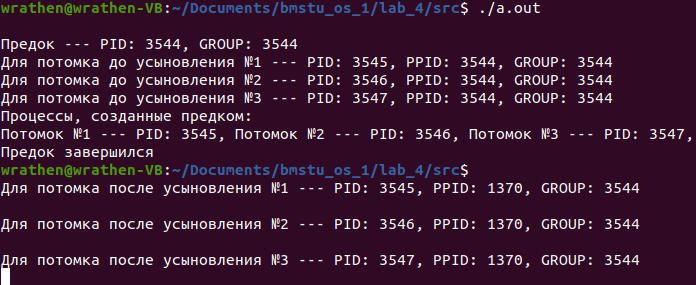
\includegraphics[width=\linewidth]{img/task_01.png}
		\caption{Демонстрация работы программы (задание №1).}
		
		\label{fig:task_01}
		
	\end{figure}

	\section*{Задание 2.}
	Предок ждет завершения своих потомком, используя системный вызов wait().
	Вывод соответствующих сообщений на экран.
	В программе необходимо, чтобы предок выполнял анализ кодов завершения потомков.
	
	\begin{lstlisting}[label=code:wait, caption=wait(), language=C]
		
	\end{lstlisting}

	\begin{figure}[H]
	
		\centering
		
		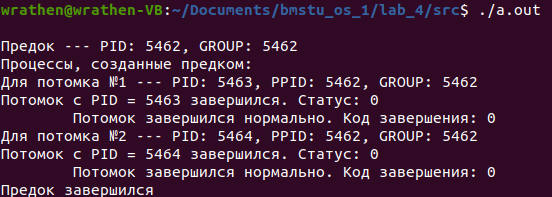
\includegraphics[width=\linewidth]{img/task_02.png}
		\caption{Демонстрация работы программы (задание №2).}
		
		\label{fig:task_02}
	
	\end{figure}

	\section*{Задание 3.}
	Потомки переходят на выполнение других программ, которые передаются
	системному вызову exec() в качестве параметра.
	Потомки должны выполнять разные программы.
	Предок ждет завершения своих потомков с анализом кодов завершения.
	На экран выводятся соответствующие сообщения.
	
	\begin{lstlisting}[label=code:exec, caption=exec(), language=C]
		
	\end{lstlisting}

	\begin{figure}[H]
	
		\centering
		
		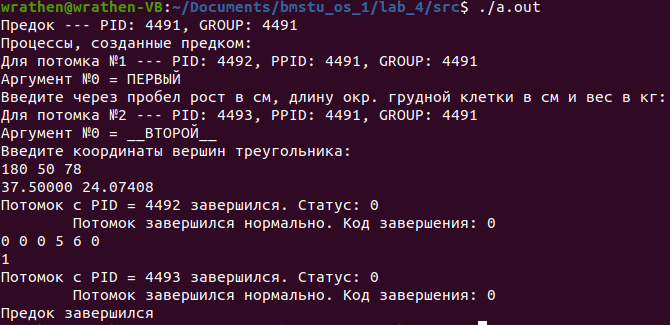
\includegraphics[width=\linewidth]{img/task_03.png}
		\caption{Демонстрация работы программы (задание №3).}
		
		\label{fig:task_03}
	
	\end{figure}

	\section*{Задание 4.}
	Предок и потомки обмениваются сообщениями через неименованный программный канал.
	Причем оба потомка пишут свои сообщения в один программный канал, а предок их считывает из канала.
	Потомки должны посылать предку разные сообщения по содержанию и размеру.
	Предок считывает сообщения от потомков и выводит их на экран.
	Предок ждет завершения своих потомков и анализирует код их завершения.
	Вывод соответствующих сообщений на экран.

	\begin{lstlisting}[label=code:pipe, caption=pipe(), language=C]
		
	\end{lstlisting}

	\begin{figure}[H]
		
		\centering
		
		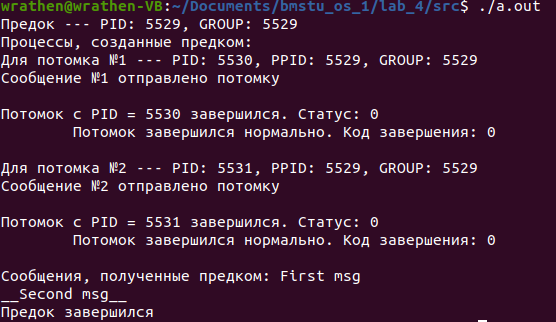
\includegraphics[width=\linewidth]{img/task_04.png}
		\caption{Демонстрация работы программы (задание №4).}
		
		\label{fig:task_04}
		
	\end{figure}

	\section*{Задание 5.}
	Предок и потомки аналогично №5 обмениваются сообщениями через неименованный программный канал.
	В программу включается собственный обработчик сигнала.
	С помощью сигнала меняется ход выполнения программы.
	При получении сигнала потомки записывают сообщения в канал, если сигнал не поступает, то не записывают.
	Предок ждет завершения своих потомков и анализирует коды их завершений.
	Вывод соответствующих сообщений на экран.
	
	\begin{lstlisting}[label=code:signal, caption=signal(), language=C]
		
	\end{lstlisting}

	\begin{figure}[H]
		
		\centering
		
		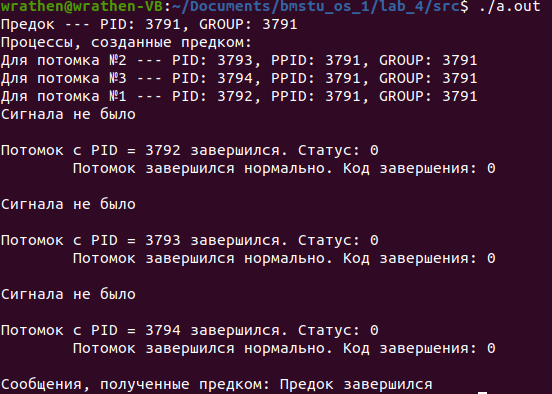
\includegraphics[width=\linewidth]{img/task_05.png}
		\caption{Демонстрация работы программы (задание №5).}
		
		\label{fig:task_05}
		
	\end{figure}
\end{document}